\documentclass[12pt]{article}
\usepackage[utf8]{inputenc}
\usepackage[T1]{fontenc}
\usepackage[french]{babel}
\usepackage{amsmath,amsfonts,amssymb}
\usepackage{fullpage}
\usepackage{graphicx}
\usepackage{hyperref}

\def\question#1{\subsection*{#1}}
\def\sec#1{\section{#1}}

\title{Les 7 merveilleuses merveilles du merveilleux monde des 7 merveilleuses couleurs}
\author{Aurèle Barrière \& Nathan Tomasset}
\date{8 mars 2016}
\setcounter{secnumdepth}{0} %for tableofcontents

\begin{document}
\maketitle
\tableofcontents
\newpage

\sec{Intoduction}
Nous présentons dans ce projet une implémentation du jeu des 7 couleurs dont les règles seront décrites plus bas. L'enjeu est d'implémenter en C le jeu, puis de créer des stratégies.
Nous proposerons une implémentation organisée, puis différentes stratégies pour jouer. Enfin, nous comparerons ces stratégies en les faisant s'affronter sur des grilles aléatoires.


\question{Règles du jeu}
Le jeu se présente comme un tableau carré de 30 case de côté (ce nombre est paramétrable dans notre implémentatoin). Initialement, il est rempli aléaoirement avec 7 ``couleurs'' (ou lettres). Dans deux angles opposés, il y a une huitième et une neuvième couleurs : celles des joueurs. Tour à tour, les joueurs choisissent une couleur parmi les 7. Toutes les cases de cette couleur et adjacente à la couleur du joueur (ou adjacente à une case qui vient de changer de couleur à ce tour par cette méthode) prennent désormais la couleur du joueur. Le but est de posséder plus de la moitié du plateau.

\sec{Organisation du projet}
Le projet est découpé de la manière suivante :

Dans un fichier header \texttt{defines.h}, on déclare les constantes pour le jeu : taille du plateau, nombre de couleurs, couleurs des joueurs. Ce fichier sera à inclure dans tous les fichiers utilisant ces constantes.
L'avantage est de pouvoir utiliser ces constantes dans tout fichier. Il faut cependant recompiler d'autres fichiers lorsqu'on change celui-ci. Ainsi, les variables globales qui sont susceptibles de changer seront déclarées globalement ailleurs.

Dans un fichier \texttt{board.c}, accompagné de son header \texttt{board.h}, on déclarera globalement les plateaux (le plateau réel, et un autre utilisé pour simuler des coups). On mettra également toutes les fonctions nécessaires à manipuler ces tableaux : \texttt{set, get} pour manipuler les valeurs, \texttt{update\_board} pour mettre ç jour un plateau après un coup, ainsi que les calculs de score ou de frontières par exemple.

Dans un fichier \texttt{strategy.c}, accompagné de son module \texttt{strategy.h}, on déclare toutes les fonction qui prennent en argument un joueur, et retournent le coup à jouer en suivant une certaine stratégie : aléatoire, gloutonne, hégémonique...

Enfin, dans un fichier \texttt{7colors.c}, on créera la fonction de jeu, et une fonction principale qui l'appelle un certain nombre de fois.

\paragraph{Remarque :} Nous avons choisi de ne pas redéfinir de types. En effet, nous aurions pu utiliser des structures pour les couleurs, les plateaux et les joueurs. Mais finalement, chacune d'entre elle ne demande rien de plus que le type de base utilisé : une couleur n'est rien de plus qu'un \texttt{char} (on affiche des lettres), un joueur n'est rien de plu qu'une autre couleur, et un plateau n'est qu'une matrice de couleurs (un vecteur de vecteurs de \texttt{char}). Renommer ces types est finalement moins intuitif que les utiliser ainsi.



\sec{Voir le monde en 7 couleurs}
\question{2.1} 
Pour initialiser le tableau de manière aléatoire, on parcourt la matrice (initialisée avec des 0), et on remplace chaque coefficient par une des 7 couleurs.

Pour obtenir ce nombre, on importe le module \texttt{stdlib}, on initialise le générateur pseudo-aléatoire avec le temps (\texttt{srand(time(NULL));}) et on prend le résultat de la fonction \texttt{rand()} modulo le nombre de couleurs.

Cependant, il faut bien initialiser l'aléatoire au début de la fonction principale, et pas à chaque partie. En effet, dans la suite on lancera plein de parties en même temps, qui seront donc identiques si lancées à moins d'une seconde d'intervalle.

Enfin, \texttt{rand()} modulo un nombre de couleurs ne produit pas un résultat avec une probabilité parfaitement uniforme, si le nombre d'entiers accessibles par \texttt{rand()} n'est pas un multiple du nombre de couleurs. En effet, soit $d$ le nombre de couleurs. Si par exemple $k\times d - 1$ couleurs sont accessibles par \texttt{rand()}, on aura $k$ entiers dont le résultat du modulo donne 0, mais seulment $k-1$ dont le résultat donne $d-1$.
Cependant, vu le petit nombre de couleurs et le grand dombre d'entiers accessibles avec \texttt{rand()}, ce n'est pas un problème significatif.

\question{2.2}
On créée une fonction \texttt{void update\_board(char player, char color, char * b)}. Elle prend en argument un joueur \texttt{player}, une couleur jouée \texttt{color} et un plateau \texttt{b}.

Elle consiste à parcourir la matrice, et si on trouve une case qui est de la couleur jouée et à côté d'une case de la couleur du joueur, on la remplace et on indique dans une variable qu'il y a eu un changement.
S'il y a eu changement, il faut recommencer le parcours de la matrice.

On pose $n$ la taille du tableau. Dans le pire cas, il faut réappliquer $n^2$ fois le parcours de matrice : à chaque parcours, il y a un changement. On a donc une complexité en $\mathcal{O}(n^4)$ dans le pire cas.

Montrons qu'il y a des fois où on doit réappliquer le parcours $\mathcal{O}(n^2)$ fois :

Dans le cas d'un serpent (voir \textsc{Figure }\ref{serpent}), si on applique l'algorithme depuis la case en bas à droite, chaque itération ne va colorier qu'une seule nouvelle case, puis se rappeler. Il va donc y avoir autant d'appels récursifs que de cases à colorier. Ce nombre de cases est un $\mathcal{O}(n^2)$ : environ la moitié de la matrice.

\begin{figure}
\center
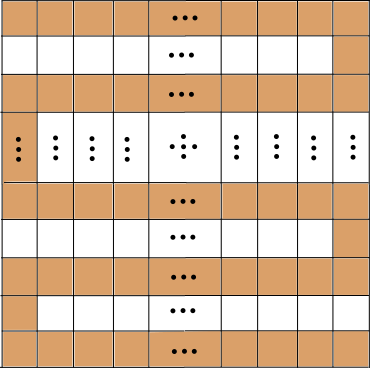
\includegraphics[scale = 0.6]{serpent.png}
\caption{Un exemple de cas pathologique pour notre algorithme}
\label{serpent}
\end{figure}

Et on ne peut pas l'appliquer plus de $n^2$ fois : à chaque appel, on a changé la matrice donc on a ajouté au moins une case.

On en déduit que la complexité au pire de cette fonction est du $\mathcal{O}(n^4)$, où $n$ est la taille du plateau de jeu.


\question{2.3}

On aurait pu implémenter une meilleure fonction de remplissage (voir \href{https://en.wikipedia.org/wiki/Flood_fill}{Flood Fill Algorithms}(lien externe)). Un des algorithmes consiste à récursivement regarder de chaque côté des cases atteintes si la case voisine est non coloriée et accessible.

On aurait ainsi pu réduire la complexité au pire à du $\mathcal{O}(n^2)$.


\sec{À la conquête du monde}
\question{3.1}
On crée donc une fonction \texttt{player\_choice}, qui demande à un joueur un caractère correspondant à une couleur. Si le caractère ne correspond pas à une de couleurs disponibles, on redemande jusqu'à obtenir un résultat convenable.

Nous n'avons pas ajouté de couleurs ou d'interface graphique. Il aurait été possible d'ajouter de la couleurs dans les fonctions \texttt{printf} de \texttt{print\_board} avec les codes couleurs ANSI. Mais il aurait fallu définir la couleur de chaque caractère. Dans notre programme, si on veut ajouter des couleurs, il n'y a qu'à modifer le \texttt{\#define NB\_COLORS} et le programme utilisera tout seul les prochaines lettres de l'alphabet.

%limites? qu'est ce qu'il va pas elle pas belle ma fonction?

\question{3.2}
On implémente la fonction \texttt{int score (char * b, int color)} qui prend en argument un plateau de jeu et la couleur d'un joueur. Elle se contente de compter le nombre de cases de cette couleur pour calculer le score d'un joueur.

On calcule la limite de score à atteindre : si $n$ est la taille du plateau, on prend $\frac{n^2}{2}$ (arrondi à la valeur supérieure).

Grâce à cette fonction, on peut donc vérifier à chaque tour si :
\begin{itemize}
\item un des joueurs a atteint la limite de score
\item les deux joueurs ont le même score qui est égal à la limite (égalité)
\end{itemize}

Ainsi, on peut mettre des conditions d'arrêt au jeu.
On peut également calculer le pourcentage en calculant $\frac{score \times 100}{n^2}$.

\sec{La stratégie de l'aléa}
\question{4.1}
Dans les fichiers de stratégies (\texttt{strategy.c, strategy.h}), on implémente une stratégie aléatoire : de la même manière qu'on choisissait une couleur aléatoire pour initialiser le plateau, on retourne une couleur aléatoire que le joueur artificiel va jouer.

\question{4.2}
On implémente une fonction \texttt{char alea\_useful\_colors(int player)} qui va opérer ainsi :

On initialise un tableau de la taille du nombre de couleurs, initialisé avec des 0. Il contiendra des booléens qui spécifieront si une couleur est utile ou non.

On parcourt le plateau de jeu. Si on tombe sur une couleur à côté d'une case occupée par le joueur, dans le tableau précédent on indiquera que cette couleur est utile (c'est à dire que le joueur progressera s'il la joue).

On caclule le nombre de couleurs utiles. On tire un nombre aléatoire plus petit que ce nombre, et on renvoie la couleur correspondante.

\paragraph{Remarque :} Il se peut que le nombre de couleurs utiles soit nul (si on a été complètement encerclé par l'adversaire). Il ne faut pas alors demander au programme de tirer un nombre aléatoire modulo 0.

\sec{La loi du plus fort}
\question{5.1}
Pour implémenter la stratégie \texttt{greedy}, nous avons utilisé le deuxième plateau \texttt{test\_board}.
Pour chacune des couleurs, on va copier \texttt{board} dans \texttt{test\_board} (avec la fonction \texttt{copy\_board()}). Puis on va simuler un coup du joueur en utilisant la fonction \texttt{update\_board} décrite plus tôt, sur le plateau \texttt{test\_board}. Pour chacun de ces tests, on calcule le score obtenu et on l'écrit dans un tableau.

Enfin, on cherche l'indice maximum de ce tableau : c'est la couleur à jouer.


\question{5.2}
Pour qu'un affrontement soit équitable, il faut alterner le premier joueur. En effet, commencer donne un avantage (pour s'en convaincre, s'imaginer le jeu à 1 ou 2 couleurs ou encore lancer des compétitions utilisant la même stratégie). On va tirer aléatoirement le premier joueur. Avec un grand nombre de parties, on devrait tendre vers un résultat équitable.

Le côté est également important. On va donc générer seulement la moitié de la matrice, puis la répliquer. La matrice est donc symétrique suivant la diagonale qui ne contient pas les positions initiales des joueurs. 

On aurait également pu faire pour chaque match le match retour, où on inverse le côté et le premier joueur.

\question{5.3}
On a fait s'affronter en 100 parties le joueur aléatoire et le joueur \texttt{greedy}.

Le joueur \texttt{greedy} les a toutes remportées.

Ensuite, on fait s'affronter en 100 parties le joueur \texttt{alea\_useful} et le joueur \texttt{greedy}.

Le joueur \texttt{greedy} les a toutes remportées.

Plus de résultats seront donnés dans la section Tournois.

\sec{Les nombreuses huitièmes merveilles du monde}

\question{6.1}
On implémente la fonction \texttt{frontier} qui, prenant en argument un joueur et un plateau, calcule le nombre de cases d'une couleur différente de celle du joueur mais à côté d'une case occupée par le joueur. 
Il s'agit de la frontière de la zone occupée par le joueur.

La stratégie consiste à maximiser cette valeur.

On implémente donc la fonction \texttt{hegemony} de la même manière que le glouton, mais en ne calculant pas le score mais bien la frontière.



\paragraph{Évaluation :}
Pour évaluer cette stratégie, on la fait s'affronter 1000 fois contre \texttt{greedy}.

\texttt{greedy} gagne 996 fois. \texttt{hegemony} gagne 4 fois. 

\sec{Stratégie générale} 
On constate que les implémentations de \texttt{starve} ou \texttt{hegemony} ressemblent fortement à celle de \texttt{greedy} : il suffit de changer la fonction à maximiser. Avec l'ordre supérieur, on peut avoir une fonction qui prend en argument une fonction à maximiser et renvoie la couleur à jouer pour maximiser cette fonction (\texttt{score} pour \texttt{greedy} et \texttt{frontier} pour \texttt{hegemony} par exemple). Il faut de plus que cette fonction ne choisisse que parmi les couleurs utiles (qui font avancer le score du joueur lorsque c'est possible), pour se garantir de la terminaison d'une partie.

On implémente donc la fonction \texttt{char general(int (*f) (char *, char), char player)}. Elle prend en argument une fonction à maximiser (\texttt{score}, \texttt{frontier} ou \texttt{personal\_space}) et un joueur et renvoie la lettre à jouer. 

Implémenter une stratégie se fait dès lors en 1 ligne :\\
\texttt{char general\_greedy(char player) \{ return general(score, player); \}}


\sec{Le pire du monde merveilleux des 7 couleurs}
\question{7.2}
On implémente la stratégie hybride \texttt{greedymony}. Il s'agit pour elle de maximiser la somme du score et de la frontière. Elle bat toutes les stratégies implémentées jusqu'à présent.

\sec{Tournois}
Dans cette section, nous comparerons les différentes stratégies en organisant des tournois de 100 parties entre chaque paire de stratégies.\\


\begin{tabular}{l|c|c|c|c|c|c|r}
strategie VS & \texttt{alea} & \texttt{alea\_useful} & \texttt{greedy} & \texttt{hegemony} & \texttt{starve} & \texttt{greedymony} & Total\\
\hline
\texttt{alea} & X & 0 & 0 & 3 & 0 & 0 & 3\\
\hline
\texttt{alea\_useful\_colors} & 100 & X & 0 & 49 & 0 & 0 & 149\\
\hline
\texttt{greedy} & 100 & 100 & X & 100 & 31 & 2 & 331\\
\hline
\texttt{hegemony} & 97 & 51 & 0 & X & 0 & 1 & 148\\
\hline
\texttt{starve} & 100 & 100 & 68 & 100 & X & 4 & 368\\
\hline
\texttt{greedymony} & 100 & 100 & 98 & 99 & 96 & X & 493\\
\hline
\end{tabular}\\

On constate que \texttt{starve} est la meilleure stratégie (elle gagne même contre \texttt{greedy} 68 à 31, et gagne 100 à 0 contre toutes les autres).

Ensuite, \texttt{greedy} ne laisse gagner personne d'autre qe \texttt{starve}.

\texttt{hegemony} n'est pas très efficace, puisqu'elle est presque équivalente à \texttt{alea\_useful\_colors}.

Enfin, la stratégie \texttt{alea} n'est vraiment pas efficace et perd presque tout le temps. 

\sec{Synthèse}
Ce projet fut pour nous l'occasion de nous intéresser à plusieurs choses.

Dans un premier temps, il fallait se fixer une architecture générale pour le projet. L'organisation en différents modules s'est révélée efficace.

Ensuite, le projet a soulevé des questions d'ordre algorithmiques (algorithmes de remplissage par exemple). Nous ne nous sommes que peu intéressé à la question de la complexité (seulement pour la mise à jour de plateau), cela ne nous semblait pas essentiel : chacune des stratégies peut être lancée une centine de fois dans un temps raisonnable (moins d'une minute). La conception de stratégies fut une partie importante de notre projet.

Cela fut également l'occasion de s'intéresser à l'ordre supérieur en C.



\sec{Bibliographie}
%j'ai pas utilisé grand chose moi. si toi t'as d'autres trucs, rajoute les

Flood Fill Algorithm : \\ \url{https://en.wikipedia.org/wiki/Flood_fill}

Higher Order in C : \\ \url{http://stackoverflow.com/questions/2535631/higher-order-functions-in-c}

Floating Point Exception : \\ \url{http://stackoverflow.com/questions/13664671/floating-point-exception-core-dump}

ANSI escape codes : \\ \url{http://stackoverflow.com/questions/3219393/stdlib-and-colored-output-in-c}








\end{document}
